% paper/sections/11_spatial_geometry.tex
% ─────────────────────────────────────────────────────────────────────────────
\subsubsection{\texorpdfstring{曲率計算の 3 経路比較}{曲率計算の3経路比較}}
\label{sec:verify_curvature}
% ─────────────────────────────────────────────────────────────────────────────

\noindent\textbf{目的：}
CSF における曲率 $\kappa$（式~\eqref{eq:curvature_2d}）の 3 計算経路の精度を比較し，
CCD 演算子の全成分（$D_x^{(10)}, D_y^{(01)}, D_{xx}^{(20)}, D_{yy}^{(02)}, D_{xy}^{(11)}$）の
総合精度を検証する．

\noindent\textbf{評価対象：}
曲率計算の 3 経路（$\phi$ 直接 / $\psi{\to}\phi$ ロジット / $\psi$ 直接）
および DCCD フィルタによる安定化．

\noindent\textbf{手順とパラメタ：}
曲率は
$\kappa = -(\phi_{xx}\phi_y^2 - 2\phi_{xy}\phi_x\phi_y + \phi_{yy}\phi_x^2)/|\bnabla\phi|^3$
により計算される．3 つの経路を比較する：
\begin{itemize}[noitemsep]
  \item \textbf{経路 A（$\phi$ 直接）：}
        真の符号付距離関数 $\phi$ に CCD を適用（理想ベースライン）．
  \item \textbf{経路 B（$\psi \to \phi$ ロジット逆変換）：}
        CLS 変数 $\psi$ からロジット逆変換
        $\phi = \varepsilon\ln[\psi/(1-\psi)]$（§~\ref{sec:newton_inversion}）で
        $\phi$ を復元（本稿採用経路）．
  \item \textbf{経路 C（$\psi$ 直接法）：}
        $\psi$ の CCD 微分値から式~\eqref{eq:curvature_psi_2d}
        （§~\ref{sec:curvature_direct_psi_cls}）で直接計算．
\end{itemize}
テスト問題：(a) 正弦波状界面 $y = 0.5 + 0.05\sin(2\pi x)$
（解析解 $\kappa = f''/(1+f'^2)^{3/2}$，$\varepsilon = 1.5h$），
(b) 円形界面（$R = 0.25$，$\kappa_\mathrm{exact} = 4$）．
格子 $N = 32$--$256$，評価指標は $L_\infty$ 誤差と収束次数．

\noindent\textbf{結果：}

\begin{table}[htbp]
\centering
\caption{正弦波状界面の曲率 $L_\infty$ 誤差収束：3 経路比較
  （$A = 0.05$，$\varepsilon = 1.5h$）}
\label{tab:curvature_sinusoidal}
\renewcommand{\arraystretch}{1.3}
\begin{tabular}{rrrrrrr}
\toprule
$N$ & A: $\phi$ 直接 & 次数 & B: ロジット経由 & 次数 & C: $\psi$ 直接 & 次数 \\
\midrule
 32 & $7.64 \times 10^{-4}$ & ---  & $7.64 \times 10^{-4}$ & ---  & $3.84 \times 10^{-2}$ & ---  \\
 64 & $2.45 \times 10^{-5}$ & 4.96 & $2.14 \times 10^{-5}$ & 5.16 & $2.19 \times 10^{-2}$ & 0.81 \\
128 & $7.72 \times 10^{-7}$ & 4.99 & $5.80 \times 10^{-6}$ & 1.88 & $2.27 \times 10^{-2}$ & $-0.05$ \\
256 & $2.42 \times 10^{-8}$ & 5.00 & $1.33 \times 10^{-5}$ & $-1.20$ & $3.59 \times 10^{-2}$ & $-0.66$ \\
\bottomrule
\end{tabular}
\end{table}

経路 A は全格子で $\Ord{h^5}$ を安定に維持し，
$D_{xy}^{(11)}$（2 方向 CCD の逐次適用）を含む曲率演算の設計精度が確認された．
経路 B は $N \leq 64$ で A とほぼ同等の精度を示したが，$N \geq 128$ では
ロジット逆変換の飽和域（$\psi \to 0, 1$）処理に起因する誤差が顕在化し，
収束が停滞ないし負の次数に転じた．
$\varepsilon = 1.5h$ のとき遷移層内の格子点数は常に約 3 点で一定であるが，
全格子点に占める飽和領域の割合が $1 - 3/N$ で増大するため，
高解像度ほど logit の高周波振動への露出が増す．
経路 C は全格子で収束しなかった（$p < 1$）．
円形界面（b）では経路 B の収束は $\Ord{h^1}$ にとどまり，
界面厚み $\varepsilon = \Ord{h}$ が精度の上界を規定した．

経路 B の高解像度での発散は，logit 飽和域で CCD が拾う高周波振動に起因する．
この対策として，経路 B 専用の後処理に DCCD 散逸フィルタ（$\varepsilon_d = 0.05$，
§~\ref{sec:dccd_filter_theory}）を適用した結果を表~\ref{tab:curvature_dccd_comparison} に示す．

\begin{table}[htbp]
\centering
\caption{経路 B 曲率誤差 $\|\kappa - \kappa_{\mathrm{exact}}\|_\infty$：
  CCD（フィルタなし）vs DCCD（$\varepsilon_d = 0.05$），円形界面 $R=0.25$}
\label{tab:curvature_dccd_comparison}
\renewcommand{\arraystretch}{1.3}
\begin{tabular}{rcccc}
\toprule
$N$ & CCD 誤差 & 次数 & DCCD 誤差 & 次数 \\
\midrule
 16 & $1.65 \times 10^{0}$  & ---    & $7.41 \times 10^{-1}$ & --- \\
 32 & $5.71 \times 10^{-2}$ & 4.86   & $2.49 \times 10^{-2}$ & 4.89 \\
 64 & $9.26 \times 10^{-5}$ & 9.27   & $1.74 \times 10^{-3}$ & 3.84 \\
128 & $2.79 \times 10^{-6}$ & 5.05   & $3.42 \times 10^{-4}$ & 2.34 \\
256 & $8.09 \times 10^{-6}$ & $-1.54$ & $7.99 \times 10^{-5}$ & $2.10$ \\
\bottomrule
\end{tabular}
\end{table}

CCD 単体では $N = 256$ で負の収束次数を示し発散に転じるのに対し，
DCCD フィルタ適用により全解像度で単調減少が実現される．
フィルタの散逸により精度は $\Ord{h^6}$ から $\Ord{h^2}$ に低下するが，
CSF モデル誤差が $\delta_\varepsilon$ の正則化幅に起因する $\Ord{h^2}$ であることを考慮すれば，
曲率の $\Ord{h^2}$ 精度は全体精度と整合的であり，安定性と引き換えに実用上の精度損失はない．
なお，HFE（§~\ref{sec:extension_pde_disc}）は $\Ord{h^6}$ を達成するため，
界面近傍の精度律速は CSF 正則化 $\delta_\varepsilon$（$\Ord{h^2}$）であり，
曲率計算経路の選択は全体精度に影響しない．
以上の結果から，本実装では DCCD フィルタ（$\varepsilon_d = 0.05$）をデフォルトで有効とする．
図~\ref{fig:curvature_3path} に 3 経路の収束曲線を示す．

\begin{figure}[htbp]
\centering
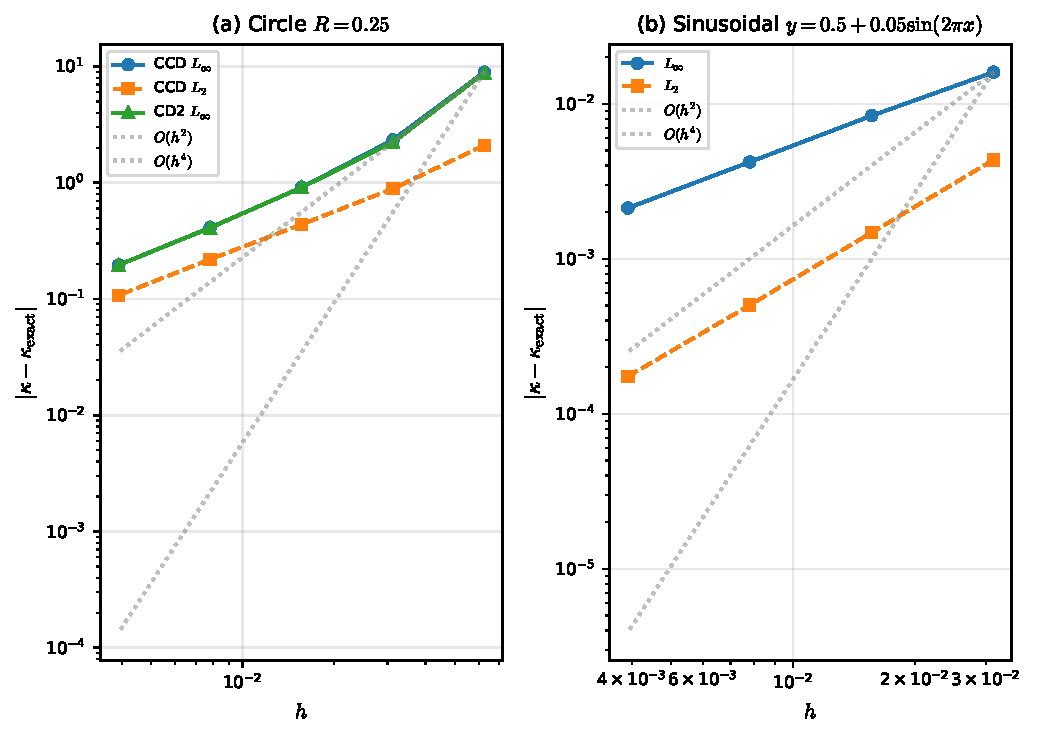
\includegraphics[width=0.92\linewidth]{figures/ch11_curvature_3path}
\caption{曲率 $\kappa$ の格子収束：3 経路比較．
  (a) 正弦波状界面：経路 A は $\Ord{h^5}$，
  経路 B は $N \leq 64$ で A と同等だが高解像度で停滞．
  (b) 円形界面（$R=0.25$）：CCD 単体は $N=256$ で発散，
  DCCD（$\varepsilon_d=0.05$）により $\Ord{h^2}$ の単調減少に安定化される．}
\label{fig:curvature_3path}
\end{figure}

\noindent\textbf{結論：}
経路 A は全格子で $\Ord{h^5}$ を安定に維持し，CCD 混合微分の設計精度が確認された．
経路 B は $N \geq 128$ でロジット飽和域の高周波振動により収束停滞；
DCCD フィルタ（$\varepsilon_d = 0.05$）で $\Ord{h^2}$ の単調収束に安定化される．
CSF 正則化 $\delta_\varepsilon$（$\Ord{h^2}$）が全体律速のため，曲率の $\Ord{h^2}$ は実用上十分である．
本実装では DCCD フィルタをデフォルトで有効とする．

% ─────────────────────────────────────────────────────────────────────────────
\subsubsection{Rhie--Chow 補正の高次精度化}
\label{sec:verify_rc_bracket}
% ─────────────────────────────────────────────────────────────────────────────

\noindent\textbf{目的：}
§~\ref{sec:rc_high_order} で導出した C/RC（CCD-enhanced RC）ブラケットが
$\Ord{h^4}$ を達成することを検証する．

\noindent\textbf{評価対象：}
RC ブラケット：標準 RC（$\Ord{h^2}$，式~\eqref{eq:rc_detection_taylor}）
vs C/RC（$\Ord{h^4}$，式~\eqref{eq:rc_crc_bracket}）．

\noindent\textbf{手順とパラメタ：}
\begin{itemize}[noitemsep]
  \item テスト関数 $p = \cos(2\pi x)\cos(2\pi y)$（$p'''$ が解析的に既知）
  \item 周期境界条件，格子 $N = 16, 32, 64, 128$
  \item 各フェイスにおける標準ブラケットと C/RC ブラケットの $L^\infty$ 誤差を計測
\end{itemize}

\noindent\textbf{結果：}

\begin{table}[htbp]
\centering
\caption{RC ブラケットの格子収束：標準 RC（$\Ord{h^2}$）vs C/RC（$\Ord{h^4}$）}
\label{tab:rc_bracket_convergence}
\renewcommand{\arraystretch}{1.3}
\begin{tabular}{rccccr}
\toprule
$N$ & $\|\text{std}\|_\infty$ & 次数 & $\|\text{C/RC}\|_\infty$ & 次数 & 改善倍率 \\
\midrule
 16 & $3.95 \times 10^{-2}$ & ---  & $1.78 \times 10^{-4}$ & ---  & $222\times$ \\
 32 & $1.00 \times 10^{-2}$ & 1.98 & $1.13 \times 10^{-5}$ & 3.98 & $889\times$ \\
 64 & $2.52 \times 10^{-3}$ & 1.99 & $7.08 \times 10^{-7}$ & 3.99 & $3557\times$ \\
128 & $6.31 \times 10^{-4}$ & 2.00 & $4.43 \times 10^{-8}$ & 4.00 & $14229\times$ \\
\bottomrule
\end{tabular}
\end{table}

標準 RC は理論通り $\Ord{h^2}$ で収束し，
C/RC は正確に $\Ord{h^4}$ を達成した（表~\ref{tab:rc_bracket_convergence}）．
$N = 128$ において C/RC は標準比約 14000 倍の改善を示す．
CCD は 1 回の求解で $p'$ と $p''$ を同時に返すため，
C/RC の実装に\textbf{追加の CCD 呼び出しは一切不要}である．
この「ゼロコスト」の精度改善は，CCD の同時微分出力という設計特性に固有の利点であり，
従来の有限差分法や有限体積法では実現できない．
図~\ref{fig:rc_bracket} に収束曲線を示す．

\begin{figure}[htbp]
\centering
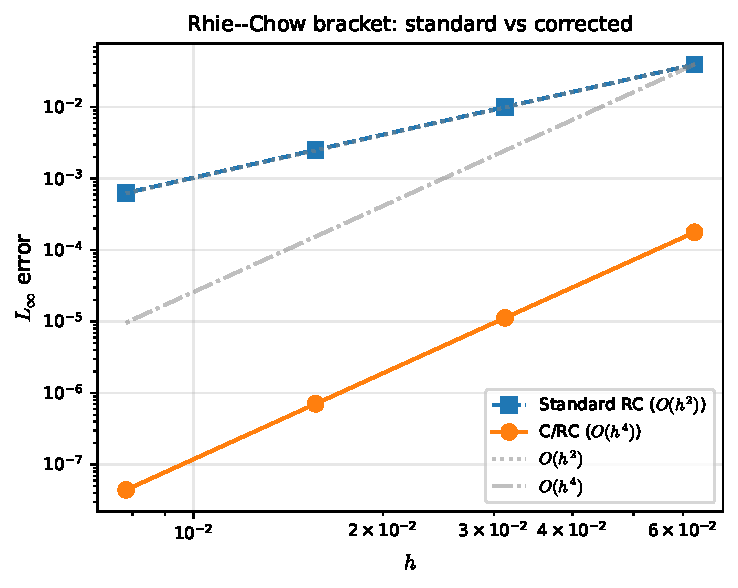
\includegraphics[width=0.88\linewidth]{figures/ch11_rc_bracket}
\caption{RC ブラケット格子収束：標準 RC（$\Ord{h^2}$）vs C/RC（$\Ord{h^4}$）．
  C/RC は CCD が同時計算する $p''$ のみを利用し，
  $N=128$ で標準比約 14000 倍の精度を達成する．}
\label{fig:rc_bracket}
\end{figure}

\noindent\textbf{結論：}
C/RC は正確に $\Ord{h^4}$ を達成し，$N = 128$ で標準比約 14000 倍の改善を示す．
CCD は 1 回の求解で $p'$ と $p''$ を同時に返すため，
追加の CCD 呼び出しは一切不要（ゼロコスト精度改善）である．

% ─────────────────────────────────────────────────────────────────────────────
\subsubsection{2D 混合偏微分の CCD 精度}
\label{sec:verify_mixed_partial}
% ─────────────────────────────────────────────────────────────────────────────

§~\ref{sec:ccd_metric} で述べた逐次 CCD 適用による
混合偏微分 $\partial^2 f / \partial x \partial y$ の精度を検証する．
テスト関数 $f(x,y) = \sin(2\pi x)\cos(2\pi y)$
（厳密解 $f_{xy} = -4\pi^2 \cos(2\pi x)\sin(2\pi y)$）に対し，
$\partial_x \to \partial_y$ と $\partial_y \to \partial_x$ の両順序で
$L_\infty$ 誤差と収束次数を測定した（$N = 16$--$256$）．

\begin{table}[htbp]
\centering
\caption{混合偏微分 $\partial^2 f / \partial x \partial y$ の格子収束}
\label{tab:mixed_partial}
\renewcommand{\arraystretch}{1.2}
\small
\begin{tabular}{rcccc}
\toprule
$N$ & $L_\infty$（周期） & 次数 & $L_\infty$（壁） & 次数 \\
\midrule
 16 & $3.23 \times 10^{-5}$ & ---  & $3.59 \times 10^{-3}$ & --- \\
 32 & $4.85 \times 10^{-7}$ & 6.06 & $1.12 \times 10^{-4}$ & 5.01 \\
 64 & $7.51 \times 10^{-9}$ & 6.01 & $3.79 \times 10^{-6}$ & 4.88 \\
128 & $1.18 \times 10^{-10}$ & 6.00 & $1.21 \times 10^{-7}$ & 4.97 \\
256 & $1.50 \times 10^{-11}$ & 2.97\textsuperscript{*} & $3.80 \times 10^{-9}$ & 4.99 \\
\bottomrule
\multicolumn{5}{l}{\footnotesize \textsuperscript{*}$N{=}256$ は丸め誤差到達．} \\
\end{tabular}
\end{table}

適用順序の交換による誤差（可換性誤差）は全条件で $\Ord{10^{-12}}$ 以下であり，
演算子の可換性が機械精度で成立している．

\noindent\textbf{結論：}
逐次 CCD 適用による混合偏微分は周期境界で $\Ord{h^{6.0}}$，
壁境界で $\Ord{h^{5.0}}$（境界スキーム律速）を達成した．
これは非対角粘性項 $\partial_y(\mu\,\partial_x u)$ の離散化に
必要な精度要件を満たしている．
